% Fast-forwarding SMV encoding: one SMV transition per entire BT tick.
\documentclass[border=6pt,tikz]{standalone}
\usepackage{tikz}
\usepackage{amsmath, amssymb}
\usepackage[T1]{fontenc}
\usepackage{lmodern}
\usetikzlibrary{arrows.meta, positioning, decorations.pathreplacing}

\tikzset{
  state/.style    = {draw, circle, fill=blue!10, minimum size=7mm, inner sep=0pt, font=\small},
  tick/.style     = {draw, rounded corners=2pt, fill=purple!15, align=center,
                     font=\small, minimum width=2.2cm, minimum height=0.75cm, inner sep=3pt},
  flow/.style     = {-{Latex[length=2mm]}, line width=0.55pt, shorten >=1pt, shorten <=1pt},
  note/.style     = {font=\scriptsize, text=black!70, align=center},
}

\begin{document}
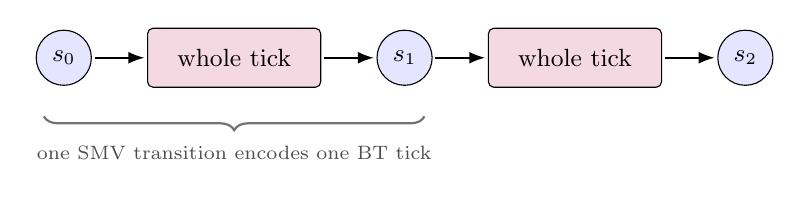
\begin{tikzpicture}[node distance=0.7cm]

\node[state] (s0) {$s_0$};
\node[tick, right=of s0] (t1) {whole tick};
\node[state, right=of t1] (s1) {$s_1$};
\node[tick, right=of s1] (t2) {whole tick};
\node[state, right=of t2] (s2) {$s_2$};

\foreach \x/\y in {s0/t1, t1/s1, s1/t2, t2/s2}
  \draw[flow] (\x) -- (\y);

\draw[decorate, decoration={brace, amplitude=5pt, mirror},
      thick, black!55]
      ([yshift=-14pt]s0.south west) -- node[below=7pt, note]
        {one SMV transition encodes one BT tick}
      ([yshift=-14pt]s1.south east);

\end{tikzpicture}
\end{document}
